\section{Introduction} \label{sec:intro}

We are currently experimenting with Google and Amazon Web Services for science platform and processing.
These services are priced to deliver compute and storage - our current model at the \gls{LDF} is also service oriented but
is not priced in the same manner making comparisons difficult.
An initial approach to a \gls{cloud} costing was outlined in \citeds{DMTN-072}; this approach was an attempt to try to cost the hardware and compare to \gls{cloud} pricing.

In this document a restructuring of \gls{LSST} operations is explored - a technology \gls{stack} underpinned by commodity services which could be provided by commercial providers or computing centers. Here we look first at how we would run something like this -- we can then leave one free variable which is the cost of the underlying compute and storage services. This will both help to
sanity check the \gls{LDF} costing and potentially allow us to have a ball park estimate for assessing commodity provider offers.


\section{Plugable service oriented architecture} \label{sec:arc}

In the Kavli workshop in Vegas (Feb 2019 \cite{2019arXiv190505116B}) we took a long term view to astronomy archives and data processing.
We suggested a layered service model as depicted in \figref{fig:CI}\footnote{The full document is here \url{https://petabytestoscience.github.io/PetaBytes-2019-04-26.pdf}}.
Our requirements are no longer unique and we have access to a wealth of open source \gls{software}, commodity hardware, and managed \gls{cloud} services (offered by commercial providers and federally-funded institutions) that are well positioned to meet the needs of \gls{LSST} \cite{2019AAS...23345706M, 2019AAS...23324505B}.


\begin{figure}
    \centering
    \includegraphics[width=1.\textwidth]{images/CI-Layers}
    \caption{An example a \gls{cyberinfrastructure} built on an Infrastructure as Code design model. Note that while this example does not have astronomy-specific tooling, our recommendations highlight the importance of developing astro-specific layers that are fully accessible to scientists in both  the application  and the graphical interface layers. \label{fig:CI}}
\end{figure}


We took \figref{fig:CI} and made a more \gls{LSST} oriented version in \figref{fig:CI-LSST}. This is pretty close to how we are currently but we do not treat the compute and storage as pure services.

\begin{figure}
    \centering
    \includegraphics[width=1.\textwidth]{images/CI-LSST}
    \caption{An example \gls{LSST}  \gls{cyberinfrastructure} built analogous to the \gls{CI} model shown in \figref{fig:CI}.}
% Original https://docs.google.com/presentation/d/16w5WVe-_xNLXWudNKqJu9IEKGDQ8oIB0eDiqWP_SUnE/edit?usp=sharing
    \label{fig:CI-LSST}
\end{figure}\

In important part of following this architecture is the ability to choose best in class components. In the science platform for example we have probably the best notebook implementation but we could possibly pick up a better portal. In processing \gls{NCSA} insist on a shared noting approach - a move to an \gls{Object Storage} could profoundly change that. It may raise other questions though on replication and redundancy. Then the shared nothing approach brings its own problems for deployment and \gls{QA}.

A more service oriented approach should allow us to move between service providers to use the best in class for our underlying services as well.  A clear model, understood by many, will make \gls{QA} an easier task as well.


Getting to operations in this model will require some rethinking in construction - construction is a big ship which is already steaming ahead so a change in course will take some effort. It is absolutely worth pursuing though.




\section{Data Production Department }\label{sec:sciops} \label{sec:dataprod}

The role of data production within \gls{LSST} is to deliver \gls{LSST}'s science products: the science images, the alert stream, the annual data releases, the science \gls{software}, and the Science Platform. In the current ops proposal not all groups required to do this are under control of Science operations.

\figref{fig:opsorg} gives a view of the Data Production teams which combine some of the old science operations  and \gls{LDF} departments. This is far more analogous to Data Management moving into operations than in the current proposal and would make for a smoother transition.

\begin{figure}
\begin{center}
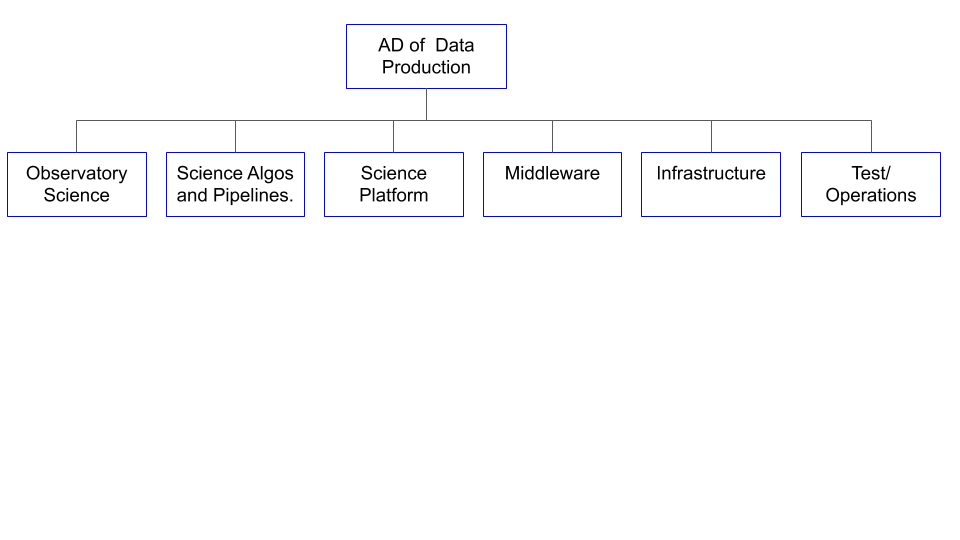
\includegraphics[width=0.9\textwidth,trim=0cm 10cm 0 0, clip]{figures/SciOpsOrg}
\caption{Possible configuration of Science Operations Department for operations of \gls{LSST} \label{fig:sciopsorg}}
\end{center}
% original https://docs.google.com/presentation/d/1wIN6Dj_rPn8TASBUkAm6_-Yh255Gz9VbwFi61t4LCFs/edit#slide=id.g55f7c0247e_0_2
\end{figure}

The \gls{FTE} counts are estimated in \tabref{tab:FTE}, which also gives the team sizes form the operations proposal for comparison.
A brief description of the teams is given in \secref{sec:teams}.
 \begin{longtable} { |p{0.3\textwidth}  |r  |r  |r  |r |} 
\caption{Size (in FTE) of the various teams in data production department with sizes including LDF teams from the proposal in the fourth column - a zero imples the team did not exist inthe proposal. \label{tab:FTE}}\\ 
\hline 
\textbf{Team}&\textbf{2023}&\textbf{2026}&\textbf{2023(P)}&\textbf{Note} \\ \hline
{Management (AD)}&{1.5}&{1.5}&{1}& \\ \hline
{Observatory Science }&{5.5}&{5.5}&{5.5}&{System performance?} \\ \hline
{Science Platform}&{6}&{6}&{6.5}& \\ \hline
{Science Algos and Pipelines}&{22}&{16}&{21}&{QA  to system performance?} \\ \hline
{Middleware}&{7.5}&{6.5}&{0}& \\ \hline
{Infrastructure}&{8}&{7}&{0}&{ } \\ \hline
{Verification/ Operations}&{5}&{4}&{0}& \\ \hline
{LDF Management (AD) }&{0}&{0}&{3}&{In infrastruture} \\ \hline
{LDF Scientific Prod. Services}&{0}&{0}&{6.75}&{In Verification/ operations} \\ \hline
{LDF ITC Security}&{0}&{0}&{8.5}&{Some in infrastructure/ middleware } \\ \hline
{LDF Prod. Services Soft.}&{0}&{0}&{7.6}&{Some in infrastructure} \\ \hline
{LDF ITC and Facilities}&{0}&{0}&{13}&{Should be in services charges} \\ \hline
\textbf{Total  FTE}&\textbf{55.5}&\textbf{46.5}&\textbf{72.85}& \\ \hline
\end{longtable}


\subsection{Teams }\label{sec:teams}
\figref{fig:sciopsorg} introduces several teams some of which were not in the original ops proposal. I  little detail is given here about each.

\subsubsection{Observatory Science}
As in the ops proposal the primary responsibility of this team is to understand the end-to-end impact of the Observatory hardware and environment on the science images and to work with the Observatory Operations department to ensure that the image quality meets requirements.

\textbf{This team may be better  in Observatory operations department }

\subsubsection{Science algorithms and pipelines}
This team is responsible to assess and assure the alert stream and annual data releases.
In the submitted proposal this includes extensive \gls{QA} to compare the data products against requirements -
this may be be better merged with Sytem Perfomance/Verification.
The main responsibility  of this team  would then be the  underlying \gls{software} pipelines themselves. Monitoring and updating the calibration plan and algorithmic implementation is also a responsibility of this team. The Calibration Support Scientist on the Observatory Science team will be responsible for monitoring the physical implementation of the calibration plan at the summit.
In \tabref{tab:FTE} this team is initially sized similarly to the AP/DRP teams in construction. There will be signifcant maintenance in the first two or three years of operations. As mentioned above there may be some consolidation with \gls{QA} activites in System Performance.

\subsubsection{Science platform  }
This team will be responsible for maintaining and evolving LSST’s user access portal, the Science Platform. This will include keeping up with evolving technologies and computing infrastructure, as well as providing basic code-base maintenance, bug fixes, and low-level response to science community and internal \gls{LSST} requests for new features.

\subsubsection{Middleware }
In a service oriented model with a layered architecture as outlined in \secref{sec:arc} it is essential to have a cross cutting team who compose and debug services.
Software such as the \texttt{butler}  is not part of the pipeline but the pipeline needs it. In house developments such as \gls{Qserv} should be covered here (1.5FTE has been included f0r this - DOE/SLAC personnel - could be 2).
This would also cover the builds and how the code interacts with the infrastructure (\secref{sec:infra}.

\subsubsection{Infrastructure, Site Reliability Engineering  } \label{ses:infra}
This is for deployment of of various systems and pipelines. Configuration is included in this. There needs to be a couple of people who manage keys/secrets
for access to commodity services. We would need a security resource as well as database expertise.  This then implies using tooling for system management as
provided by e.g. \gls{AWS} console.

In general an \gls{SRE} team is responsible for the availability, latency, performance, efficiency, change management, monitoring, emergency response and capacity planning of their services \cite{Beyer:2016:SRE:3006357}.

This team would include paying for a liaison at any service provider e.g. Google Professional Services or a Service Manager at \gls{NCSA}. (2FTE calculated)

\subsubsection{Verification/Operations }
This team will take and verify new releases for operations before they are deployed to the operations system. They will monitor the operational system to make sure it is functioning - they should have some science knowledge to know it is actually working properly as opposed to not just giving errors. A team of 4 should be able to handle this.
Some support for this is assumed from IN2P3 .





\subsection{Service budget}

If we assume we do not reduce the operations budget then the total cost of the \gls{LDF} services is
the difference in \gls{FTE} and the non labor costs for computer purchases.
This is calculated in \tabref{tab:Services} .

 \begin{longtable} { |p{0.3\textwidth}  |r  |r |} 
\caption{Estimate of service budget/cost using \gls{FTE} and non-labor costs from the proposal.  \label{tab:Services}}\\ 
\hline 
\textbf{}&\textbf{FTE}&\textbf{Cost K\$} \\ \hline
{Annual labour diff from \tabref{tab:FTE}}&{17.35}&{\$4,338} \\ \hline
{Non labour hardware (average of all years - NOT CORRECT NUMVER)}&{}&{\$8,000} \\ \hline
\textbf{Total}&\textbf{}&\textbf{\$12,338} \\ \hline
\end{longtable}


\textbf{ These non labor numbers need to come out of the proposal sheets - I only had a \gls{PDF} and did not try to do this properly. It should exclude the BASE hardware and Chilean archive hardware budgets.}


We would still require some hardware on the mountain and the base in Chile where we would potentially still keep a copy of the raw data.


The  LSST data volumes are in  \tabref{tad:sizes}.

\input{images/sizetab}



The compute estimates are a little more difficult to extract in \tabref{tab:Inputs} from \citeds{DMTN-072}
an estimate is made in terms of FLOPs.

\tiny \begin{longtable} { |p{0.22\textwidth}  |r  |r  |r  |r  |r  |r |} 
\caption{Various inputs for deriving costs \label{tab:Inputs}}\\ 
\hline 
\textbf{Year}&\textbf{2017}&\textbf{2018}&\textbf{2019}&\textbf{2020}&\textbf{2021}&\textbf{2022} \\ \hline
{FLOPs Needed Total (no Alerts)}&{9.48261E+19}&{1.00E+19}&{1.00E+19}&{9.48261E+19}&{1.00E+19}&{4.74131E+20} \\ \hline
{Time to Process days}&{252.0}&{365.0}&{365.0}&{252.0}&{365.0}&{252.0} \\ \hline
{Time to Process seconds}&{21772800.0}&{31536000.0}&{31536000.0}&{21772800.0}&{31536000.0}&{21772800.0} \\ \hline
{Instantaneous GFLOP/ s}&{4355.255691}&{3.17E+02}&{3.17E+02}&{4355.255691}&{3.17E+02}&{21776.27846} \\ \hline
{Instantaneous GFLOP/ s (inc Alerts)}&{4355.255691}&{3.17E+02}&{3.17E+02}&{30025.25569}&{2.60E+04}&{21776.27846} \\ \hline
{Disk Space TB}&{1000}&{1000}&{1000}&{10000}&{20000}&{30000} \\ \hline
{I/ O for year TB}&{10}&{100}&{3000}&{30000}&{60000}&{90000} \\ \hline
{Base numbers }&{Ecyc }&{FLOP}&{GFLOP}&&& \\ \hline
{LDM-138 DR1,2 Data Rel sheet row 1}&{155.17}&{4.26718E+20}&{426717500000}&&& \\ \hline
{LDM-138 DR3 Data Rel sheet row 2}&{348.76}&{9.5909E+20}&{959090000000}&&& \\ \hline
{LDM-138 Alert Instananeous}&{0.00023434}&{25670000000000}&{25670}&&& \\ \hline
{Alert Total, assuming 275k visits/ year}&{64.4435}&{1.7722E+20}&{177219625000}&&& \\ \hline
\textbf{Total Yr1 (inc DAC)}&\textbf{}&\textbf{4.74131E+20}&\textbf{474130555556}&&& \\ \hline
{}&{Optimistic}&{Pessimistic}&&&& \\ \hline
{Moore Factor Proc}&{0.7}&{0.9}&&&& \\ \hline
{Kryder Factor Disk}&{0.8}&{0.9}&&&& \\ \hline
\end{longtable} \normalsize


\section{Other implied changes to the current operations proposal}
Notably missing from \figref{fig:sciopsorg} is \gls{QA}. Currently \gls{QA} is spread across  three
 departments - the suggestion here is to place all \gls{QA} activities under the survey performance department. Consolidation
of the \gls{QA} activities in one department may allow for some personnel saving.

The data release team in science operations would require a verification scientist 
(this may be 0.5FTE) while the \gls{SDQA} and Semantic scientists may move to QA in survey science.

All data facility work, be it with a partner or in commercial \gls{cloud} should be 
firmly under science operations - hence there is no \gls{LDF} department and no associate director 
for \gls{LDF} as depicted in \figref{fig:opsorg}.\footnote{This is  in line with AMCL recommendations}

\begin{figure}
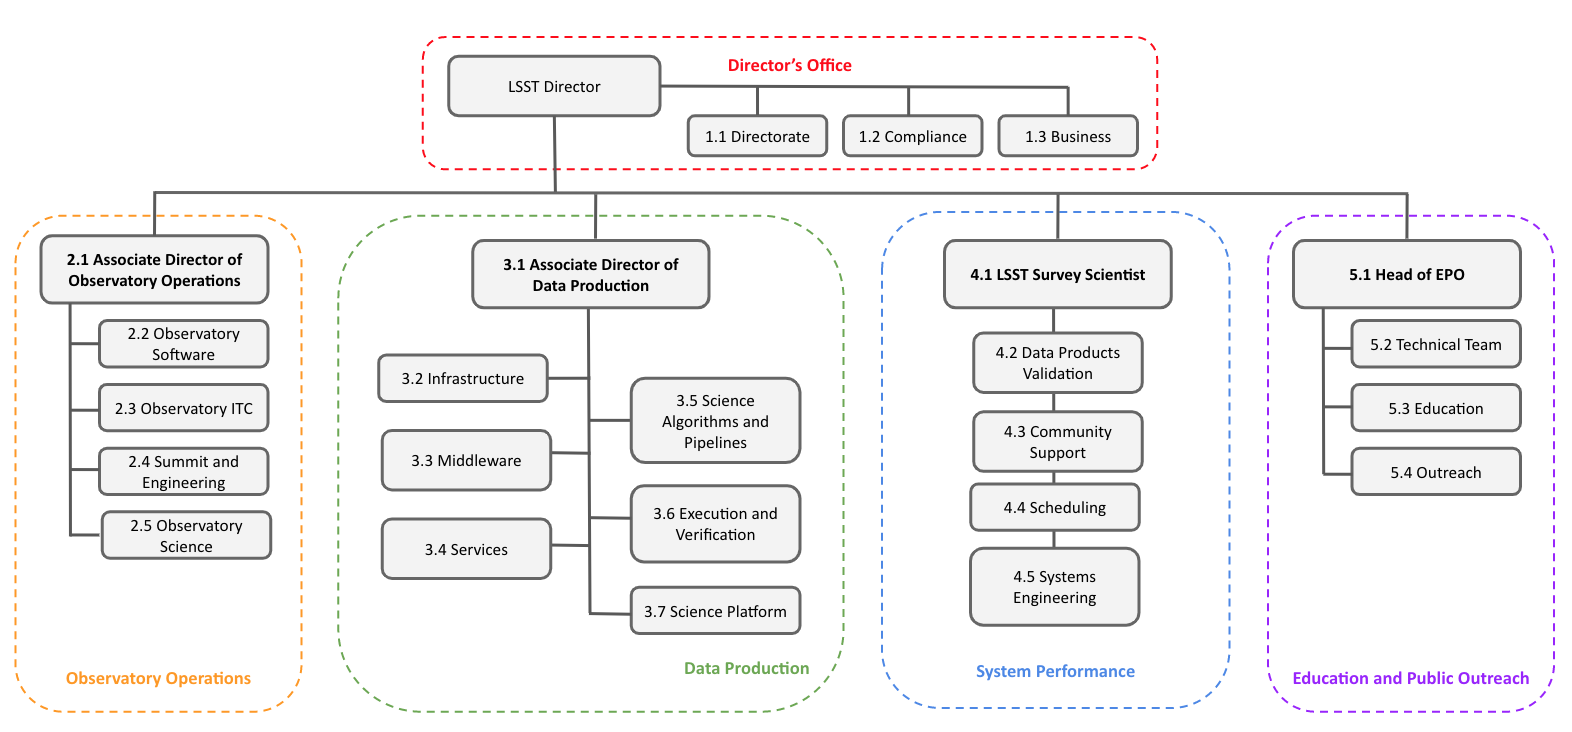
\includegraphics[width=1.0\textwidth]{figures/OpsOrg2}
\caption{Possible new organisation chart for \gls{LSST}  operations \label{fig:opsorg}}
% original https://docs.google.com/presentation/d/1H7sn92FXDa9-cgFrizgN12KI3Br60Ffbk4qA8fxCvMg/edit#slide=id.g5132af8469_0_81
\end{figure}

%\textbf{NOTE: I have said before communications should report directly to the director - in \figref{fig:opsorg} there is NO communications.}

ITC and facilities (\figref{fig:opsorg}) in this model should come from \gls{NCOA}  logically also this does not belong in data production but at a higher level its for the entire org, the observatory already has its own \gls{ITC} group so they are good.

There are still some developments in \gls{NCSA} such as \gls{DAQ} forwarders which would need to be included in possibly the observatory \gls{software}.

There are other developments \gls{DBB} which could be replaced by commodity services like Amazon \gls{S3} which includes replications and reliability.



\section{Conclusion}\label{sec:conclusion}
 A restructuring of operations would  give more transparent cost, allow for a better comparison to commodity pricing for many services and would
yield considerable savings.

